\documentclass{beamer}

\usepackage[latin1]{inputenc}
\usepackage[T1]{fontenc}
\usepackage[danish]{babel}
\usepackage{sudoku}
\usepackage{hyperref}
\usepackage{lastpage}

\date{20. juni 2007}
\author[Emil Erik Hansen \newline \newline Julian M�ller \newline \newline Klaes Bo Rasmussen \newline \newline Steen Nordsmark Pedersen]{Emil Erik Hansen \and Julian M�ller \and Klaes Bo Rasmussen \and Steen Nordsmark Pedersen}
\institute{Gruppe 4}
\title{Sudoku til undervisningsbrug}
\titlegraphic{
\includegraphics[width=30mm]{billeder/welcome.png}}

\setcounter{tocdepth}{2}

\mode<presentation>
{ \usetheme[hideothersubsections, right]{Goettingen} }

\AtBeginSection[]
{
   \begin{frame}
       \frametitle{Overblik}
       \tableofcontents[currentsection]
   \end{frame}
}

\begin{document}

\begin{frame}
\titlepage
\end{frame}

\section{Analyse}

\section{Design af l�sning}

\subsection{Overordnet design}
\begin{frame}
\frametitle{Overordnet design}

\begin{itemize}
	\item Eksekverbar JAR-fil
	
	\item Platforme
		\begin{itemize}
			\item Windows
			\item Linux
		\end{itemize}
		
	\item Applet i browser
		\begin{itemize}	
			\item Internet Explorer 5.5+
			\item Mozilla Firefox 1.5+
		\end{itemize}
	
	\item Java 1.5
	
	\item Gamle versioner med vilje
\end{itemize}

\end{frame}

\subsection{Vigtige aspekter}
\begin{frame}
\frametitle{Vigtige aspekter}
\begin{itemize}
	\item Gr�nsefladen
		\begin{itemize}
			\item Simpel, tillokkende
		\end{itemize}

	\item Sudokugenerator
		\begin{itemize}
			\item L�sbare sudokuer
			\item Flere sv�rhedsgrader
			\item H�j hastighed
		\end{itemize}

	\item Nemt at udvide
		\begin{itemize}
			\item Designparadigmer
			\item Interfaces
		\end{itemize}
\end{itemize}

\end{frame}

\subsection{Model-View-Control (MVC)}
\begin{frame}
	\frametitle{Model-View-Control}
	\begin{itemize}
		\item Seperation af data, logik og udseende
		\item Tre moduler
	\end{itemize}
	
	\pause
	
	\begin{figure}[hp]
		\centering
			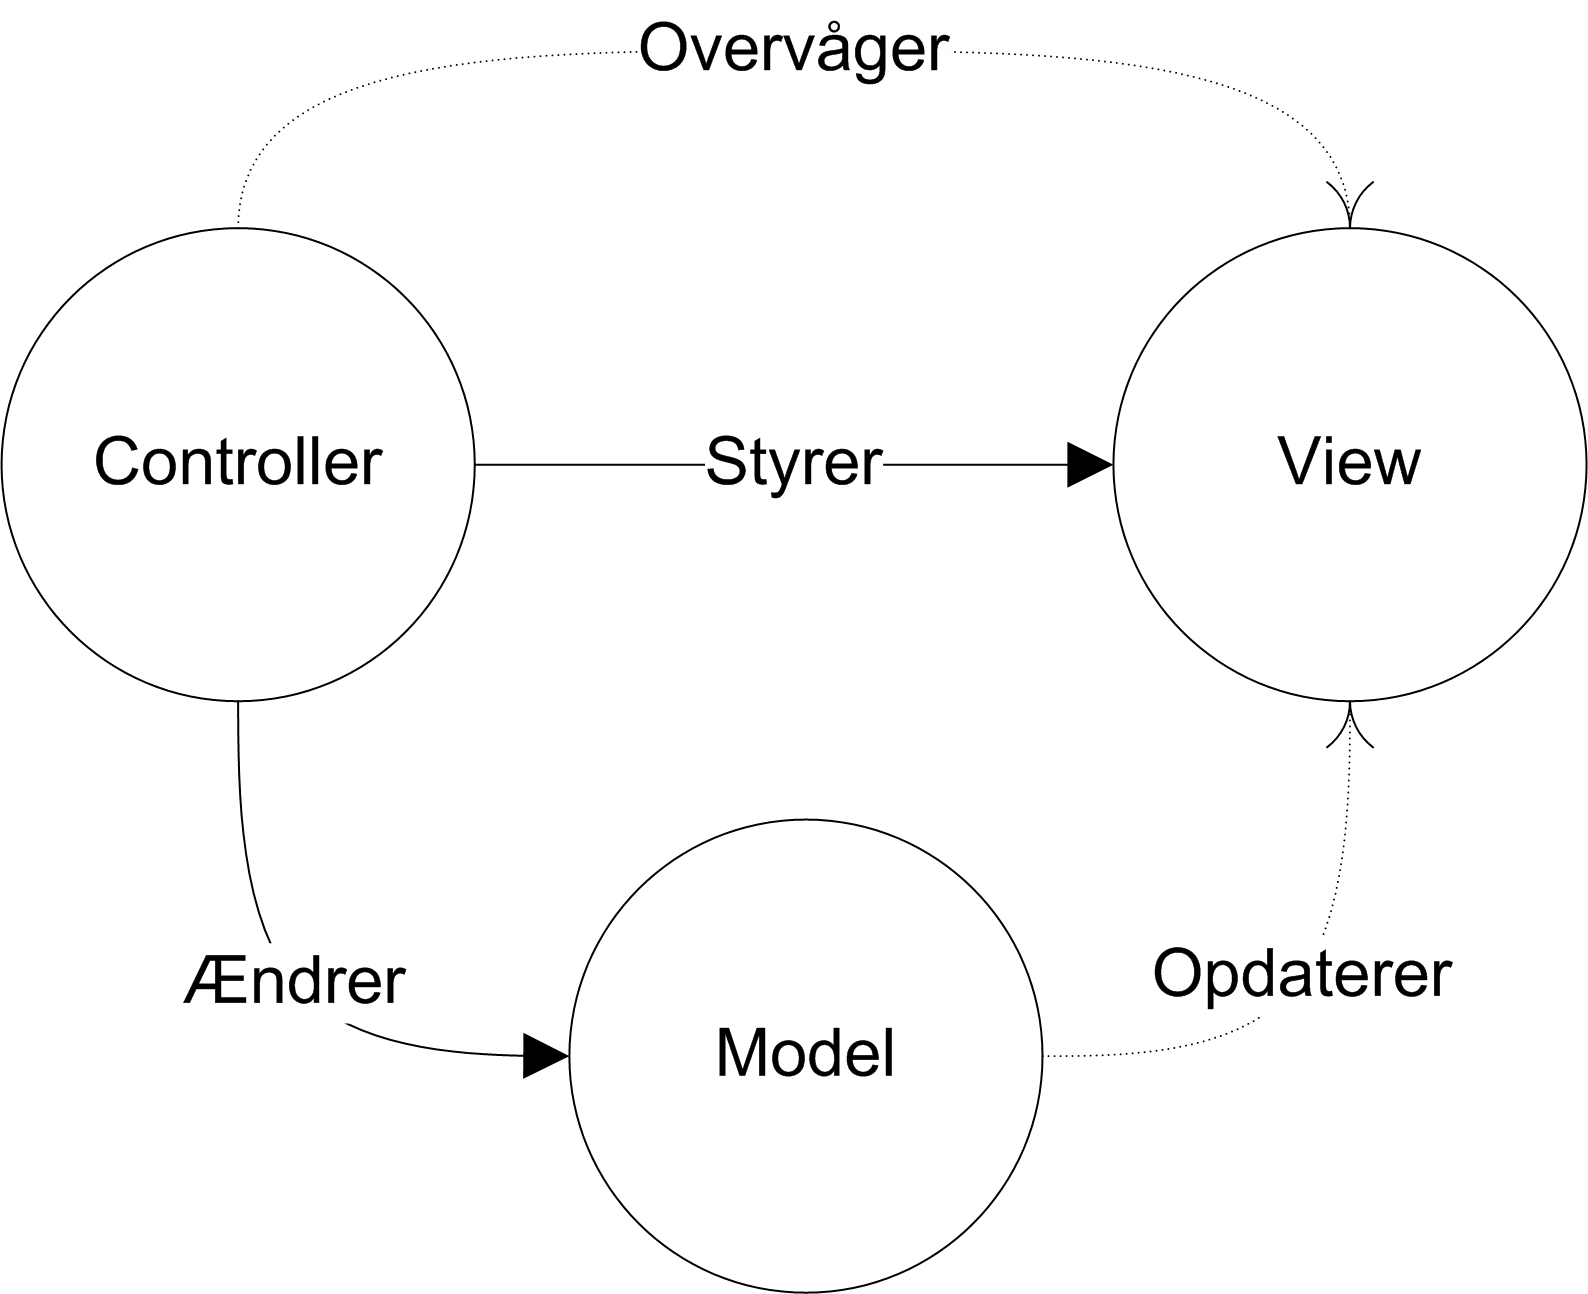
\includegraphics{billeder/MVC.png}
		\caption{Model-View-Controller samspillet}
	\end{figure}
\end{frame}

\subsubsection{Model}
\begin{frame}
	\frametitle{Model-View-Control (forts.)}
	
	\begin{itemize}
		\item Model
		\pause
			\begin{itemize}
				\item Sudokugenerator
				\item Sudokul�ser
				\item Hj�lpefunktion
				\item Indstillinger
				\item Matematiske metoder til beregning p� sudoku
			\end{itemize}
	\end{itemize}		
\end{frame}

\subsubsection{View}
\begin{frame}
	\frametitle{Model-View-Control (forts.)}
	
	\begin{itemize}
		\item View
			\begin{itemize}
				\item Spilleplade
				\item Maskot
				\item Knapper og baggrunde
				\item Vinduer
			\end{itemize}
	\end{itemize}	
\end{frame}

\subsubsection{Control}
\begin{frame}
	\frametitle{Model-View-Control (forts.)}
	
	\begin{itemize}	
		\item Control
			\begin{itemize}
				\item Initialiserer programmet eller applet
				\item S�rger for at knapper o.l. g�r noget
				\item S�rger for at View viser det rigtige
				\item Opdaterer Model
			\end{itemize}
	\end{itemize}
\end{frame}

\subsection{Observer og Observable}
\begin{frame}
	\frametitle{Observer og Observable}
	
	\begin{itemize}
		\item Mulighed for overv�gning
		\item Logik flyttes
	\end{itemize}
	
	\begin{itemize}
		\item Vores implementering
		\item Muligheder
	\end{itemize}
\end{frame}

\section{Teknisk beskrivelse}

\section{Grafisk design}
\subsection{Brugergr�nseflade}
\begin{frame}
	\frametitle{Brugergr�nseflade del 1}
	
	\begin{itemize}
		\item Intuitivt
		\item Farvevalg
	\end{itemize}
	
		\begin{figure}[hp]
		\centering
			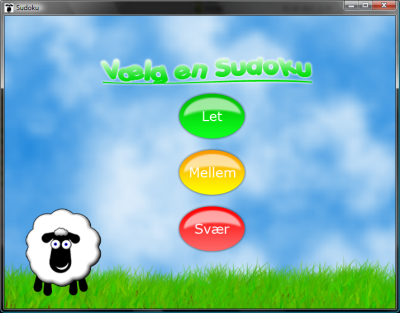
\includegraphics[width=50mm]{billeder/Vaelg_Sudoku.png}
		\caption{Startsk�rmen i programmet.}
	\end{figure}
	
		\begin{itemize}
		\item Maskotten Dolly
	\end{itemize}
\end{frame}

\begin{frame}
	\frametitle{Brugergr�nseflade del 2}
	
	\begin{itemize}
		\item Sudoku spillet
		\item Talvalg og inaktive felter
	\end{itemize}
	
		\begin{figure}[hp]
		\centering
			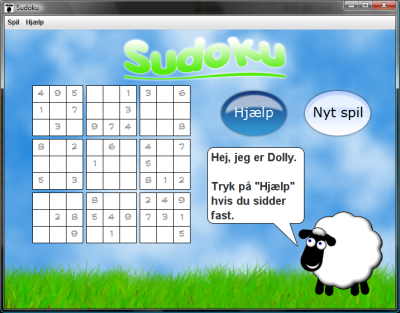
\includegraphics[width=50mm]{billeder/Spilleplade.png}
		\caption{Spillepladen.}
	\end{figure}
\end{frame}

\begin{frame}
	\frametitle{Brugergr�nseflade del 3}
	
	\begin{itemize}
			\item ``Tillykke''-sk�rmen
			\item Statistik
		\end{itemize}
	
		\begin{figure}[hp]
		\centering
			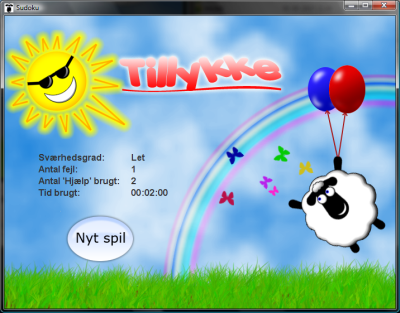
\includegraphics[width=50mm]{billeder/Tillykke.png}
		\caption{``Tillyke''-sk�rmen i programmet.}
	\end{figure}
\end{frame}

\section{Test}

\subsection{Funktionstest}


\subsection{Brugertest}

\end{document}